 \documentclass[12pt]{article}
%\usepackage[portuguese]{babel}
\usepackage{natbib}
\usepackage{url}
\usepackage[utf8x]{inputenc}
\usepackage{amsmath}
\usepackage{graphicx}
\graphicspath{{images/}}
\usepackage{parskip}
\usepackage{fancyhdr}
\usepackage{vmargin}
\setmarginsrb{1.5 cm}{2.5 cm}{1.5 cm}{2.5 cm}{1 cm}{1.5 cm}{1 cm}{1.5 cm}
\usepackage{hyperref}
\hypersetup{
    colorlinks=true,
    citecolor=black,
    filecolor=black,
    linkcolor=black,
    urlcolor=black
}
\let\oldhref\href
\renewcommand{\href}[2]{\oldhref{#1}{\bfseries#2}}

\usepackage[bottom]{footmisc}
\usepackage{caption}
\DeclareCaptionFormat{sanslabel}{#3}%
\usepackage[section]{placeins}
\usepackage{xcolor}
\definecolor{light-gray}{gray}{0.95}
\usepackage{listings}
\lstset{basicstyle=\ttfamily,
  showstringspaces=false,
  commentstyle=\color{red},
  keywordstyle=\color{blue},
  backgroundcolor=\color{light-gray},
  breaklines=true,
  extendedchars=true,
  literate={é}{{\'e}}1
}
\lstset{aboveskip=15pt,belowskip=15pt}
\usepackage[autostyle]{csquotes}  
\def\labelitemi{--}
\usepackage{enumitem}
\setlist{nosep}
\usepackage{booktabs}

\title{Tutorial 1}								% Title
%\author{}								% Author
\date{\today}											% Date

\makeatletter
\let\thetitle\@title
%\let\theauthor\@author
\let\thedate\@date
\makeatother

\pagestyle{fancy}
\fancyhf{}
%\rhead{\theauthor}
\lhead{\thetitle}
\cfoot{\thepage}

\begin{document}

%%%%%%%%%%%%%%%%%%%%%%%%%%%%%%%%%%%%%%%%%%%%%%%%%%%%%%%%%%%%%%%%%%%%%%%%%%%%%%%%%%%%%%%%%

\begin{titlepage}
	\centering
    \vspace*{0.5 cm}
    
\includegraphics[scale = 0.3]{logo4.png}\\[1.0 cm]
    \textsc{\LARGE \newline\newline UNIX 101}\\[2.0 cm]
	\textsc{\Large or "How to feel like a true hack3r"}\\[0.5 cm]
	\rule{\linewidth}{0.2 mm} \\[0.4 cm]
	{ \huge \bfseries \thetitle}\\
	\rule{\linewidth}{0.2 mm} \\[1.5 cm]
	
%	\begin{minipage}{0.5\textwidth}
%		\begin{flushleft} \large
%			\emph{Professor:}\\
%			Renan E P Lima\\
%            Departamento de Matemática\\
%			\end{flushleft}
%			\end{minipage}~
%			\begin{minipage}{0.4\textwidth}
%           
%			\begin{flushright} \large
%			\emph{Grupo:} \\
%			Gabriel P Crestani\\
%           Victor R Sales\\
%		\end{flushright}
%        
%	\end{minipage}\\[2 cm]
	
	
    \thedate
    
    
    
	
\end{titlepage}

%%%%%%%%%%%%%%%%%%%%%%%%%%%%%%%%%%%%%%%%%%%%%%%%%%%%%%%%%%%%%%%%%%%%%%%%%%%%%%%%%%%%%%%%%

\tableofcontents
\pagebreak

%%%%%%%%%%%%%%%%%%%%%%%%%%%%%%%%%%%%%%%%%%%%%%%%%%%%%%%%%%%%%%%%%%%%%%%%%%%%%%%%%%%%%%%%%

\section{Foreword}

\subsection{Objective}
This tutorial should teach you the basics of working with a terminal. You are not expected to fully assimilate everything that this document is about in details, but you should at least understand the basics of every notion. You can come back to this tutorial whenever you want to refresh your mind.

If you work thoroughfully, at the end of this tutorial, you should know:

\begin{itemize}
\item What the syntax of a command is
\item A few useful commands
\item How to navigate in a filesystem
\item How to create, edit and remove files
\item What is a packet manager and how to use one
\item How to create your own executable scripts
\end{itemize}

Even thought you may already have a bit of knowledge on the topics we will study, we will start again from the beginning. It will help you assimilate completely the basics and provide you a stronger basis to learn new things.

\subsection{Preliminary setup}

You are going to need a UNIX-like operating system for this tutorial.
A Linux distribution is preferred but a Mac can also do the job (OS X is a variant of FreeBSD).

If your operating system is a Windows, the safest way is for you to start a virtual machine running a Linux distribution although you could also run the Windows Subsystem for Linux\footnote{\url{https://en.wikipedia.org/wiki/Windows_Subsystem_for_Linux}}. It allows one to run the latest versions of Ubuntu on a Windows 10 machine, but it is still new, so at your own risk!



\section{Terminal and shell}

\subsection{A terminal?}

To be precise, a \textit{terminal emulator} is a program reading the user's keyboard input.

Inside a terminal runs a \textit{shell}. This is a program that works in pair with a terminal. The shell's job is basically to read the text it is given as input and interpret it into actual actions.
Of course, the shell does not understand random text input; it tries to interpret what the user inputs into commands.
We will detail the syntax of a command later on.

\begin{figure}[!h]\centering\captionsetup{}
   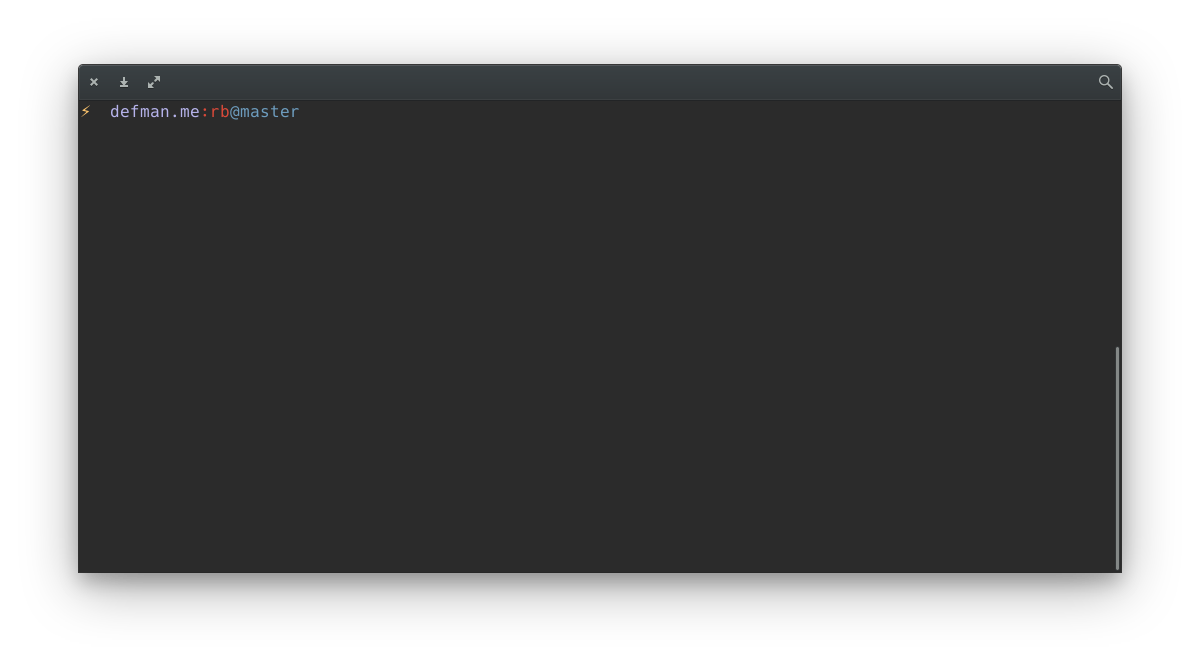
\includegraphics[scale = 0.20]{terminal.png}
   \caption{This is what a terminal looks like}
\end{figure}

\subsection{Opening a terminal}

Let us try it now! Open a new terminal. On a fresh Ubuntu install, the shortcut is \texttt{Ctrl+T}. On a Mac, you should be able to launch one by first pressing \texttt{Cmd+Space} and then typing "Terminal".
You should be prompted with a window like the following:

\begin{lstlisting}[language=bash]
nico@nico-VirtualBox:~$
\end{lstlisting}

This is called the prompt. Typically, the \texttt{\$} at the end of the line represents the position where you start typing text.
From now on, the examples on this tutorial will all start with that \texttt{\$}.

\subsection{Anatomy of a command and manual}

First, we will call the command \texttt{ls} (list). This program, susprinsigly, allows one to get the \textit{list} of files in the current directory.

\begin{lstlisting}[language=bash]
$ls
Desktop Documents Downloads Music Pictures Public Templates Videos
\end{lstlisting}

That is great! But wait, do not leave yet, there is more. One can alter a command's behavior by adding arguments. See after:
\begin{lstlisting}[language=bash,breaklines=true]
$ls /
bin/    home/            lost+found/  root/  sys/      vmlinuz.old@
boot/   initrd.img@      media/       run/   tmp/
cdrom/  initrd.img.old@  mnt/         sbin/  usr/
dev/    lib/             opt/         snap/  var/
etc/    lib64/           proc/        srv/   vmlinuz@
\end{lstlisting}

Here, the first argument of the command was \texttt{/}. Thus, the command \texttt{ls} changed its behavior to list the root directory (\texttt{/}) instead of the current directory.

Last but not least, arguments can take the form of flags. One can recognize a flag because it begins by a dash (\texttt{-}). In the following example, we use the flag \texttt{-l}:

\begin{lstlisting}[language=bash]
$ls -l /
total 119
drwxr-xr-x   2 root root  4096 déc.  23 19:02 bin/
drwxr-xr-x   4 root root  3072 déc.  23 19:07 boot/
drwxrwxr-x   2 root root  4096 févr. 26  2018 cdrom/
drwxr-xr-x  22 root root  4400 janv.  4 22:38 dev/
drwxr-xr-x 153 root root 12288 déc.  23 22:52 etc/
drwxr-xr-x   4 root root  4096 févr. 26  2018 home/
lrwxrwxrwx   1 root root    33 déc.  23 19:05 initrd.img -> boot/initrd.img-4.15.0-43-generic
lrwxrwxrwx   1 root root    33 déc.  23 19:05 initrd.img.old -> boot/initrd.img-4.15.0-33-generic
drwxr-xr-x  25 root root  4096 sept.  5 09:17 lib/
drwxr-xr-x   2 root root  4096 févr. 26  2018 lib64/
drwx------   2 root root 16384 févr. 26  2018 lost+found/
drwxr-xr-x   5 root root  4096 mai   15  2018 media/
drwxr-xr-x   7 root root  4096 juin  20  2018 mnt/
drwxr-xr-x   6 root root  4096 juin   4  2018 opt/
dr-xr-xr-x 290 root root     0 janv.  4 19:41 proc/
drwx------  11 root root  4096 janv.  4 21:49 root/
drwxr-xr-x  34 root root  1100 janv.  4 19:42 run/
drwxr-xr-x   2 root root 12288 déc.  23 19:02 sbin/
drwxr-xr-x   5 root root  4096 sept.  1 19:16 snap/
drwxr-xr-x   2 root root  4096 févr. 15  2017 srv/
dr-xr-xr-x  13 root root     0 janv.  4 19:42 sys/
drwxrwxrwt  15 root root 20480 janv.  5 02:28 tmp/
drwxr-xr-x  12 root root  4096 mars  29  2018 usr/
drwxr-xr-x  14 root root  4096 févr. 15  2017 var/
lrwxrwxrwx   1 root root    30 déc.  23 19:05 vmlinuz -> boot/vmlinuz-4.15.0-43-generic
lrwxrwxrwx   1 root root    30 déc.  23 19:05 vmlinuz.old -> boot/vmlinuz-4.15.0-33-generic
\end{lstlisting}

That is quite a lot of information! The option \texttt{-l} allows one to get much more information than with a simple \texttt{ls}.

To check out the full list of possible arguments you can use with ls, use the command \texttt{man ls}.
The \texttt{man} command gives information about the command given as argument. From now on, this will be your best friend. \textbf{Before asking for help, always check out the manual}. The answer to your question will, in 90\% of the cases, be findable inside.

Also, at the top of every man page is the prototype (\textit{"synopsys"}) of the command. It will help you figure out how you should call it, in which order the arguments can be put and which arguments are mandatory for the command to run.

\subsection{Demystifying "commands"} \label{demystifying_commands}

Actually, the term \textit{command} is not accurate.

When one launches the command \texttt{ls}, the program at location \texttt{/bin/ls} is executed by the shell. Then, in this case, entering in the shell \texttt{ls} is the same as entering \texttt{/bin/ls}, but faster.

Using \texttt{which ls} tells you where the program \texttt{ls} is located.
One simply has to list the content of the directory \texttt{/bin} to verify that \texttt{ls} is a program that lies there:

\begin{lstlisting}[language=bash]
$ls -l /bin
total 13044
(...)
-rwxr-xr-x 1 root root   56152 mars   2  2017 ln
-rwxr-xr-x 1 root root  111496 sept. 22  2016 loadkeys
-rwxr-xr-x 1 root root   48128 mars  26  2019 login
-rwxr-xr-x 1 root root  453856 juin  27 17:49 loginctl
-rwxr-xr-x 1 root root  105136 mars  21  2019 lowntfs-3g
-rwxr-xr-x 1 root root  126584 mars   2  2017 ls
-rwxr-xr-x 1 root root   77280 oct.  10 11:34 lsblk
(...)
\end{lstlisting}

By the way, \texttt{which} is also a program, so entering \texttt{which which} in the shell works!

However, some commands do not depend on the programs on your system. They are contained within the shell tool set, literally built in. Thus, we call then... built-in commands\footnote{\href{https://unix.stackexchange.com/questions/11454/what-is-the-difference-between-a-builtin-command-and-one-that-is-not}{This question}'s responses might give you a deeper understanding of the difference between these two types of commands}.

Before ending this section, it is important to understand that there is no black magic in UNIX systems. The shell does not magically know where to look for the program \texttt{ls} when an user inputs that. There is a special variable that the shell keeps track of: the \texttt{PATH}.

\begin{lstlisting}[language=bash]
$echo $PATH # Show the content of PATH variable
/usr/local/sbin:/usr/local/bin:/usr/sbin:/usr/bin:/sbin:/bin:/usr/games:/usr/local/games
\end{lstlisting}

It references all of the location where binaries are supposed to sit, separated by a colon (\texttt{:}).
When the shell encounters a non-builtin command, it will simply check in all of the locations referenced in the path, one by one, if there is a program named as the command. If there is one, it will start it; if not, it will raise an error.

\subsection{Why the command line?}

Now you may be wondering why bother using fastidious commands to simply show a list of files. It would be way simpler to use a graphical tool like Mac's Finder or Windows's file explorer!

Well, even though it is more complicated to do basic things, the diversity of options shipped with every command allows one to do much more than simply with a GUI.
It is also possible to combine options, widening the range of possibilites.
The philosophy of UNIX is for each command to be able to do a limited set of things, but to do it perfectly.

A few other reasons as to why knowing how to work on a command line is important:
\begin{itemize}
\item Many technical actions cannot be done graphically, a lot of software engineering/sysadmin programs only have a command line interface (CLI)
\item Scripts are essential to computer engineering and are nothing but a list of sequential commands to execute
\item Thanks to their variety of options, command line programs allow one to run complex tasks in a simple line. Imagine how tiresome it would be to copy just one kind of files from one huge directory to another using Window's file manager
\end{itemize}


\section{Core utilities}

Now that you have an idea on how to use commands and most importantly on where to find documentation, let us dig into the basics.
In this section, you will learn how to navigate in your filesystem and how to alter it.
Do not forget to take a look at the manual in case of doubt.

\subsection{Filesystem navigation}

Let us review the commands that allow you to move around your filesystem.

\subsubsection{ls ("list")}

This is an easy one, we have just learned about it the last section. Remember to use the manual for things that you do not know how to do.
Try to:
\begin{enumerate}
\item List the content of the current directory, including the hidden files\footnote{In UNIX, hidden files' filenames begin with a "."}. What do you think the \texttt{.} and \texttt{..} directories refer to?
\item List the content of \texttt{/etc}. What do you think is inside?
\item List the content of \texttt{/etc} and all of its subdirectories in one command
\end{enumerate}

\subsubsection{pwd ("print working directory")}

This command is super simple. It simply gives you the full path of your shell's current directory.

Try it! Open a new terminal and type \texttt{pwd}.
\begin{lstlisting}[language=bash]
$pwd
/home/nicolas
\end{lstlisting}
This is what is called your \textit{home}. Every user of the computer has its own home directory, where he can put his files.

\subsubsection{cd ("change directory")}

This command allows you to move from one directory to another. It is similar to double-clicking on the icon of a directory.


\begin{enumerate}
\item Try to open the man for this command. What happens?

\texttt{cd} is a builtin command (cf. \ref{demystifying_commands}). \texttt{man} works only with actual programs installed on your system. To get help for this kind of commands,
you can use \texttt{help my\_command}.
\item What is the difference between writing \texttt{cd /bin} and \texttt{cd bin}?
\item Move anywhere in your filesystem. Then, type \texttt{cd} without any argument. Where are you now?
\item Move anywhere in your filesystem. Then, type \texttt{cd ~}. Where are you now?
\item Move to \texttt{/etc}, then move to \texttt{/usr}. Finally, type \texttt{cd -}. Where are you now?
\end{enumerate}


\subsection{File manipulation}

Great, we know how to move in our filesystem. Let us start manipulating files and directories!

\subsubsection{mkdir ("make directory")}

As its name indicates it, this command allows one to create a new directory.
\begin{enumerate}
\item Move to your home directory and create a directory named \texttt{code}
\item Move to your home directory and, with a single \texttt{mkdir} command, create the two directories \texttt{code/python} and \texttt{code/python/exo\_1}
\end{enumerate}

\subsubsection{rmdir ("remove directory")}

As we just saw how to \textit{make} a directory, this allows one to \textit{remove} one.
Note that this command only works on empty directories.

\subsubsection{cp ("copy")}

This one allows one to copy files and directories from a directory to another.
\begin{enumerate}
\item Create a new directory and copy the file \texttt{/etc/hostname} inside
\item Create a new directory and recursively copy all of the files and directories from \texttt{/etc} inside. Can you guess why warnings are printed to the screen?
\end{enumerate}

Also, remember this in the previous section?

\begin{quote}
\textit{Imagine how tiresome it would be to copy just one kind of files from one huge directory to another using Window's file manager}
\end{quote}

It can be done super easily using \texttt{cp} combined with a wildcard\footnote{\url{https://www.shell-tips.com/2006/11/04/using-bash-wildcards/}}.

\begin{lstlisting}[language=bash]
$mkdir /tmp/mdr
$cp /etc/*.conf /tmp/mdr/
$ls --format=single-column /tmp/mdr/
adduser.conf
apg.conf
appstream.conf
brltty.conf
ca-certificates.conf
debconf.conf
deluser.conf
fuse.conf
fwupd.conf
gai.conf
hdparm.conf
host.conf
idmapd.conf
insserv.conf
kernel-img.conf
kerneloops.conf
ld.so.conf
lftp.conf
libao.conf
libaudit.conf
logrotate.conf
ltrace.conf
mke2fs.conf
mtools.conf
nsswitch.conf
pam.conf
pnm2ppa.conf
popularity-contest.conf
request-key.conf
resolv.conf
rsyslog.conf
sensors3.conf
signond.conf
smi.conf
sysctl.conf
ucf.conf
updatedb.conf
usb_modeswitch.conf
\end{lstlisting}

\subsubsection{mv ("move")}

The \texttt{mv} command allows one to move a file or directory somewhere else. It is similar to a "Cut\&Paste".
It can also be used to rename a file.

\begin{enumerate}
\item Create a new directory, copy the file \texttt{/etc/hostname} inside and rename it \texttt{file1}.
\item Duplicate \texttt{file1} and create another directory. With one command, move both files to that new directory
\end{enumerate}

\subsubsection{rm ("remove")}

This command allows one to remove a file from the filesystem.

Be careful when using it as you will not be prompted a warning when you are attempting to delete a file. What is more, there is no "Trash bin" in the command line world. Once a file is deleted, it is gone for good.

\begin{enumerate}
\item Remove every file and directory you put in your home directory in the previous exercises
\end{enumerate}

\subsubsection{touch}

Last but not least, the command \texttt{touch} allows one to change the time of last modification of a file. Honestly, it is not very useful, but it is possible to use it to create empty files:

\begin{lstlisting}[language=bash]
$mkdir test
$cd test
$touch hello
$ls
hello
$
\end{lstlisting}


\subsection{Peek inside files}

We have manipulated directories and files but we still do not know how to show their content. Let us dig into this now.

\subsubsection{cat ("catenate", it seems)}

This command simply displays the content of the files given as argument.

\begin{enumerate}
\item Read the content of \texttt{/etc/os-release}. What do you think this file refers to?
\item Read the content of \texttt{/etc/hosts} and \texttt{/etc/hostname} in just one command
\item Using an option of cat, find out how many lines are inside the file \texttt{/etc/services}\footnote{There is a command called \texttt{wc} which is specialized in counting the number of lines, but let us not use this one for now :)}
\end{enumerate}

\subsubsection{head \& tail}

These two commands are similar to \texttt{cat} but only display the beginning (head) or the end(tail) of a file. It can be useful to read the beginning or the end huge files.
The number of lines displayed default to 10, but it can be changed with an option. 

\begin{enumerate}
\item Display the first 20 lines of \texttt{/etc/inputrc}
\item Display the last two bytes of \texttt{/etc/hosts}. Display the last byte of \texttt{/etc/hosts}. Why do you think you get this result? Using the \texttt{-E} option of cat, identify what the last byte of this file is
\end{enumerate}

\subsubsection{less}

This program is a pager. It allows one to look into a file without having to load all of its content into memory (hence the name, it \textit{paginates}). It is extremely useful when dealing with huge files, like servers logs.
This pager is invoked using \texttt{less path\_to\_file} and provides the user a way to:
\begin{enumerate}
\item Navigate in between the lines: press \textit{up} and \textit{down} arrow keys or \textit{j} and \textit{k})
\item Move to top or bottom: press \textit{g} or \textit{G}
\item Search for the occurrences of a work: press \textit{/}, write your word, press \textit{Enter} and navigate through the occurrences using \textit{n} and \textit{N}
\item And many more...
\end{enumerate} 

Use \textit{h} to get some help inside the pager and press {\textit{q}} to leave.

The design of \texttt{less} might make you think of \texttt{man}. That is because \texttt{man} is also a pager. The shortcuts we just went through can also be used when reading a man page! Useful when trying to look for specific information :)


\section{File editor, package manager and permissions}

Great, we have seen many things. But we are still not able to edit files. Let us remediate to this

\subsection{File editor}

There are many file editors\footnote{We will not discuss IDEs in this tutorial} available in Linux and Mac OS. Pick one in the following list.

\begin{description}
	\item[vim:] This is a highly configurable text editor. It is lightweight and designed to optimize writing code. There is an incredible set of shortcut and commands to your disposal, which allow you to do tons of advanced things.
	
	Also, it is an in-terminal software, meaning that you will stay in the same terminal window as the one you currently are in when you invoke it. 

	Still, beware, because it is not an easy task to get started with using \textbf{vim}. The controls are not-intuitive\footnote{Many are similar to the pager's}, so it is a pain to get started with it.
	\item[nano:] Just like \textbf{vim}, \textbf{nano} is an in-terminal software. It is simpler to use but provides less features.
	\item[gedit:] It is a primitive GUI editor bundled with GNOME\footnote{\url{https://en.wikipedia.org/wiki/GNOME_Shell}}. It aims at simplicity and is perfect for performing simple editing tasks.
	\item[Atom:] A GUI editor. It provides a beautiful and clean interface. One can also install plugins and themes to customize it. It is described as a \textit{hackable text editor}: combine plugins and your configuration to make it your own.
	
	Only downside: it is a bit slow at times.
	\item[sublimeText:] Very similar to Atom, but in general faster.
\end{description}

If you do not feel comfortable learning how to use an in-terminal text editor like vim, my advice for you is to pick either \textbf{Atom} or \textbf{sublimeText}.
However, it is important for you to know the basics of either \textbf{vim} or \textbf{nano}, because sometimes, you do not have access to a graphical interface and an in-terminal editor is necessary.

\subsection{Installation}

Chances are that \textbf{nano} and \textbf{gedit} are already installed in your system. To check, simply use the command \texttt{which}. This command allows one to get the location of the program.

\begin{lstlisting}[language=bash]
$which nano
/bin/nano
$which vim
$
\end{lstlisting}

As you can see, nano is installed in my system while vim is not.
This is the perfect opportunity to learn how to install programs in UNIX-like systems!

\subsubsection{Package manager}

A package manager is a tool allowing one to install, uninstall and update \textit{packages}.
A package is simply an archive containing source code and/or applications.

Ubuntu's default packet manager is \texttt{apt}. Mac OS does not have one, but you can install \texttt{brew}\footnote{\url{https://brew.sh/}}.

Keep in mind that not every program is available in the official package repositories. Hence, \textbf{Atom} and \textbf{sublimeText} are not available on Ubuntu repositories. In the following example, we will use \texttt{apt} to install vim. We will detail in the next subsection how to manually install a software.

A look at the man indicates us that we can install a package using \texttt{apt install package\_name} (\texttt{brew install package\_name} for Mac users).

\begin{lstlisting}[language=bash]
$apt install vim
E: Could not open lock file /var/lib/dpkg/lock-frontend - open (13: Permission denied)
E: Unable to acquire the dpkg frontend lock (/var/lib/dpkg/lock-frontend), are you root?
$
\end{lstlisting}

Oops, that did not work. It seems that we do not have sufficient permissions! We can bypass this using the \texttt{sudo} command. It allows one to launch commands as administrator (\textit{root}). Keep this in mind, we will talk about permissions in the next section.

\begin{lstlisting}[language=bash]
$sudo apt install vim
[sudo] password for nico: 
Reading package lists... Done
Building dependency tree       
Reading state information... Done
The following additional packages will be installed:
  vim-runtime
Suggested packages:
  ctags vim-doc vim-scripts
The following NEW packages will be installed:
  vim vim-runtime
0 upgraded, 2 newly installed, 0 to remove and 297 not upgraded.
Need to get 6 589 kB of archives.
After this operation, 32,0 MB of additional disk space will be used.
Do you want to continue? [Y/n]
\end{lstlisting}

Here, we enter \texttt{Y} and press enter to validate. Informational text is displayed and we get control back. Let us check that we installed \texttt{vim} correctly:

\begin{lstlisting}[language=bash]
$which vim
/usr/bin/vim
$
\end{lstlisting}

Great, it worked!

Refer to the manual for more information on \texttt{apt} (how to remove packages, how to upgrade software and how to update the list of available packages).

\subsubsection{Installing packages manually}

So, let us say we want to install \textbf{Atom} on a fresh Ubuntu system.

\begin{lstlisting}[language=bash]
$sudo apt install atom
[sudo] password for nicolas: 
Reading package lists... Done
Building dependency tree       
Reading state information... Done
E: Unable to locate package atom
$
\end{lstlisting}

Here, the error message is pretty explicit: \texttt{apt} could not find a package containing the program \texttt{atom}. We will have to install it ourselves.

Going to their official site, we can download a \texttt{.deb} file: \url{https://atom.io/download/deb}.
Once saved to our system, we will simply call the following \texttt{dpkg}\footnote{Actually, \texttt{apt} uses \texttt{dpkg} underneath the calls to its high-level API} command to install it.

\begin{lstlisting}[language=bash]
$ls Downloads
atom-amd64.deb
$sudo dpkg -i Downloads/atom-amd64.deb
[sudo] password for nicolas: 
Selecting previously unselected package atom.
(Reading database ... 364547 files and directories currently installed.)
Preparing to unpack Downloads/atom-amd64.deb ...
Unpacking atom (1.33.1) ...
Setting up atom (1.33.1) ...
Processing triggers for desktop-file-utils (0.22-1ubuntu5.2) ...
Processing triggers for bamfdaemon (0.5.3~bzr0+16.04.20180209-0ubuntu1) ...
Rebuilding /usr/share/applications/bamf-2.index...
Processing triggers for gnome-menus (3.13.3-6ubuntu3.1) ...
Processing triggers for mime-support (3.59ubuntu1) ...
$which atom
/usr/bin/atom
\end{lstlisting}

There you have it!

\subsubsection{Finally, editing a file!}


Now that your favorite editor is installed, simply invoke it with the name of the file you want to create:

\begin{lstlisting}[language=bash]
$cd Documents
$vim my_document
(...editing...)
$cat my_document 
Hello!
$
\end{lstlisting}


\subsection{Permissions and root user}

Remember in last section when we encountered a \textit{Permission denied} error? Let us explain what happened here.

\subsubsection{File permissions}

\begin{lstlisting}[language=bash]
$apt install vim
apt install vim
E: Could not open lock file /var/lib/dpkg/lock-frontend - open (13: Permission denied)
E: Unable to acquire the dpkg frontend lock (/var/lib/dpkg/lock-frontend), are you root?
$
\end{lstlisting}

It seems that, for some reason, \texttt{apt} needed to open the file \texttt{/var/lib/dpkg/lock-frontend}.

In UNIX-like systems, each file is attributed a set of permissions:
\begin{itemize}
	\item read (\textbf{r}, value \textbf{4}): this permission allows one to get the content of a file or to list the content of a directory
	\item write (\textbf{w}, value \textbf{2}): this allows one to edit the content of a file\footnote{Not renaming or destruction of a file. Permissions for this kind of operation are a bit more complex: \url{https://unix.stackexchange.com/a/230508}}
	\item execute (\textbf{x}, value \textbf{1}): this last permission allows one to execute a file if it is a program or a script. If it is a directory, this means that the user can move to it
\end{itemize}

There is thus a total of 8 different possible combinations:
 
\begin{table}[ht]
\centering
\begin{tabular}[t]{lcc}
\toprule
&Textual representation &Numerical representation\\
\midrule\
No permission&\textbf{---}&\textbf{0}\\
Execute-only&\textbf{--x}&\textbf{1}\\
Write-only&\textbf{-w-}&\textbf{2}\\
Write \& execute&\textbf{-wx}&\textbf{3} (2 + 1)\\
Read-only&\textbf{r--}&\textbf{4}\\
Read \& execute&\textbf{r-x}&\textbf{5} (4 + 1)\\
Read \& write&\textbf{rw-}&\textbf{6} (4 + 2)\\
Read \& write \& execute&\textbf{rwx}&\textbf{7} (4 + 2 + 1)\\
\bottomrule
\end{tabular}
\caption{The 8 file permissions combinations}
\end{table}%

\subsubsection{File ownership}

In UNIX-like systems, we say that a file is owned by a user. If the user \texttt{nicolas} creates a file, he will be the owner.

Linking that distinction to the mechanism of file permissions, a file in your filesystem is supposed to have three triplets of permissions: one for the user which owns it, one for the group of the user which owns it and lastly one for every other user of the system.

This "triple triplet" is in the following order: \textit{user, group, others}.

\begin{figure}[!h]\centering\captionsetup{}
   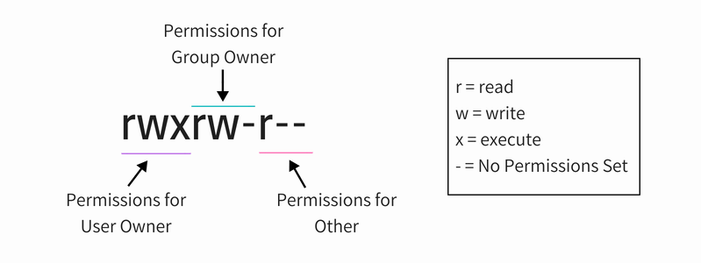
\includegraphics[scale = 0.65]{permissions.png}
   \caption{Permissions of a file}
\end{figure}


\subsubsection{Showing a file's permissions}
The \texttt{-l} option of \texttt{ls} allows one to show files in the \textit{long-listing format}, including the owner of the file and the file permissions.

\begin{figure}[!h]\centering\captionsetup{}
   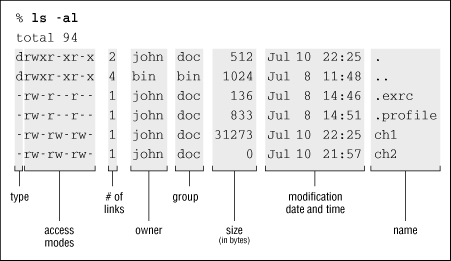
\includegraphics[scale = 0.65]
{llformat.png}
   \caption{Long listing format}
\end{figure}


Let us try:
\begin{lstlisting}[language=bash]
$touch my_file
$ls -l my_file 
-rw-rw-r-- 1 nicolas nicolas 0 janv.  7 01:48 my_file
\end{lstlisting}

Here, the owner is \texttt{nicolas} and so is the group of the owner. The access rights say that I can read or modify the file and so can the members of the group \texttt{nicolas}. However, users not in the group \texttt{nicolas} only have read access.

Let us see another example:

\begin{lstlisting}[language=bash]
$which mkdir
/bin/mkdir
$ls -l /bin/mkdir
-rwxr-xr-x 1 root root 76848 mars   2  2017 /bin/mkdir*
\end{lstlisting}

The file \texttt{/bin/mkdir}, which I invoke using the command \texttt{mkdir}, is owned by the \texttt{root} user (i.e the administrator). The \texttt{root} user can read it, modify it and execute it. The members of its group can only read it and execute it. I can also read it and execute it. Let us verify:

\begin{lstlisting}[language=bash]
# Read permission
$head -c 4 /bin/mkdir
ELF$

# Write permission
$ rm /bin/mkdir 
rm: remove write-protected regular file '/bin/mkdir'? y
rm: cannot remove '/bin/mkdir': Permission denied

# Execute permission
$/bin/mkdir /tmp/my_new_directory
$ls -d /tmp/my_new_directory
/tmp/mydir/
$
\end{lstlisting}

Knowing this and the fact that \texttt{sudo my\_command} launches \texttt{my\_command} as the \texttt{root} user, can you troubleshoot why we could not open the file \texttt{/var/lib/dpkg/lock}?

\begin{lstlisting}[language=bash]
ls -lh /var/lib/dpkg/lock
-rw-r----- 1 root root 0 janv.  6 22:32 /var/lib/dpkg/lock
\end{lstlisting}

\subsubsection{Modifying permissions}

The file owner and the root user can both modify the permissions of a file. One calls the \texttt{chmod} command for that.

There are different ways to invoke \texttt{chmod}. The following lines are examples that will help you understand how one changes the three triplets of permissions for a file.


\begin{description}
	\item[Octal representation:] The first digit represents the right of the owner, the second digit the rights of its group and the last one the rights associated to all the other users

\begin{lstlisting}[language=bash]
# Set read-only rights for everybody
$chmod 444 my\_file
# Set read-write-execute rights for the user, read-write for the users of its group and read-only for other users
$chmod 764 my\_file
\end{lstlisting}

	\item[Symbolic representation:] With symbolic representation, you do not set permissions, you add (\textbf{+}) or remove (\textbf{-}) them to the \textbf{u}ser, \textbf{g}roup and/or \textbf{o}thers.

\begin{lstlisting}[language=bash]
# Add write permission for the other users
$chmod o+w my_file
# Remove execute permission for owning user and its group
$chmod ug-x my_file
# Add read-write permissions to user and its group and read for others
$chmod ug+rw o+r my_file
# If invoked without u, g or o, it defaults to ugo: this adds the execute permission on the file for all users
$chmod +x my_file
# This is similar to the following (a stands for all)
$chmod a+x my_file
\end{lstlisting}
\end{description}

It is also possible to modify the file owner using the command \texttt{chown}. We will not go throught this one though.


\subsection{Creating your own programs}

Did you think creating your own scripts was a difficult task? Actually, you have pretty much all the cards in your hands right now to create your very own programs. You know how to create a file, edit it and set it executable.

\subsubsection{A shell script}

Let us create our very own shell script now! Using your favorite text editor, create a file called \texttt{my\_ls.sh}.

Although this is not absolutely needed, it is a good practice to start a script with a \textit{shebang}. A \textit{shebang} is a line indicating which program is supposed to run the script. It is made of a sharp (\texttt{\#}), a bang (\texttt{!}) and the full path of the program which will run the script.

A shell script can be run using \texttt{bash}, the shell that we have been using since the beginning of this tutorial, or any other shell (\texttt{sh}, \texttt{zsh}, etc).

First of all, locate bash's full path. Open a terminal and type the following:
\begin{lstlisting}[language=bash]
$which bash
/bin/bash
\end{lstlisting}

Then, write the shebang at the beginning of your script:

\begin{lstlisting}[language=bash]
#! /bin/bash
\end{lstlisting}

Then, you can start building your script. A shell script is simply a list of commands. Shell being a script language, there exists conditional statement, loops and many much more. For now, we have not studied the subject enough, so let us simply call a simple command with fancy options: a recursive \texttt{ls} with long-listing format, also displaying hidden files.

\begin{lstlisting}[language=bash]
#! /bin/bash

ls -Rahl
\end{lstlisting}

That's it. We have our first program, a \texttt{ls} on steroids! Now, the syntax to launch a program is as follows\footnote{It also is possible to directly call the executable: \texttt{/bin/bash my\_ls.sh} or \texttt{/bin/python3 my\_python\_program.py}}:

\begin{lstlisting}[language=bash]
$./my_ls.sh
bash: ./my_ls.sh: Permission denied
\end{lstlisting}

Oops, something is wrong. We forgot to make the file executable. Easy, let us use \texttt{chmod}.

\begin{lstlisting}[language=bash]
$chmod +x my_ls.sh 
$./my_ls.sh
(huge output)
\end{lstlisting}

It works! :)

\subsubsection{A python script}

You have seen how to write a shell script, but it was not that useful nor impressive, since you may not have sufficient knowledge in this scripting language.

Python being an interpreted language, one can write Python scripts just as Shell scripts. There is below the code for a number guessing game. With basic notions of Python, you should be able to get what it is doing easily. We will make a script out of this snippet, and run it inside the terminal.

First, install Python3:

\begin{lstlisting}[language=bash]
# For Ubuntu users
$sudo apt install python3-pip
\end{lstlisting}

\begin{lstlisting}[language=bash]
# For Mac OS users
$brew intall python3
\end{lstlisting}

Now, find the absolute path to Python3's binary:

\begin{lstlisting}[language=bash]
$which python3
/usr/bin/python3
\end{lstlisting}

Finally, create a file named \texttt{guessing\_game.py} and paste the following code snippet inside. Do not forget to change the shebang if it does not fit the location of your python3 binary.

\begin{lstlisting}[language=python]
#! /usr/bin/python3

# The random package is needed to choose a random number
import random

# Define the game in a function
def guess_loop():
    # This is the number the user will have to guess, chosen randomly in between 1 and 100
    number_to_guess = random.randint(1, 100)
    print("I have in mind a number in between 1 and 100, can you find it?")

    # Replay the question until the user finds the correct number
    while True:
        try:
            # Read the number the user inputs
            guess = int(input())

            # Compare it to the number to guess
            if guess > number_to_guess:
                print("The number to guess is lower")
            elif guess < number_to_guess:
                print("The number to guess is higher")
            else:
                # The user found the number to guess, let's exit
                print("You just found the number, it was indeed", guess)
                return
        # A ValueError is raised by the int() function if the user inputs something else than a number
        except ValueError as err:
            print("Invalid input, please enter an integer")

# Launch the game
guess_loop()
\end{lstlisting}

Save the file, make it executable using \texttt{chmod} and launch it:

\begin{lstlisting}[language=bash]
$./guessing_game.py 
I have in mind a number in between 1 and 100, can you find it?
50
The number to guess is higher
75
The number to guess is lower
63
The number to guess is lower
57
The number to guess is lower
53
The number to guess is higher
55
The number to guess is higher
56
You just found the number, it was indeed 56
$
\end{lstlisting}

There it is! You actually \textit{ran Python code}. It might look like nothing, but believe it or not, what servers do all around the world is nothing but run code like this snippet\footnote{Maybe stuff more useful than a guessing game, but still!}.

You can now write your own Python applications and run them in your \textit{own} environment. You do not have to rely on online platforms anymore.

Regarding Bash and Linux, there are still many things to learn, but this is a good start. Chances are that you will not assimilate everything from this tutorial, it is pretty dense after all. But do not hesitate to come back to this resource every once in a while to refresh your mind :)


\end{document}
